\documentclass[12pt, a4paper]{article}

\usepackage[utf8]{inputenc}
\usepackage[T1]{fontenc}
\usepackage[russian]{babel}
\usepackage[oglav,spisok,boldsect, figwhole]{./style/fn2kursstyle}
\graphicspath{{./style/}{./figures/}}
\usepackage{float}%"Плавающие" картинки
\usepackage{multirow}
\usepackage{subcaption}
\usepackage{comment}
\usepackage{soul,color}
\usepackage{makecell}
\usepackage{amsfonts}
\usepackage{float}%"Плавающие" картинки

%Параметры титульника
\title{Численное моделирование напряженно-деформированного\\состояния твердого тела}
\group{ФН2-62Б}
\author{Г.А.~Швецов}
\supervisor{М.П.~Галанин}
\date{2023}
\begin{document}
	\newcommand{\pl}{\partial}
	\maketitle
	\tableofcontents
	
	\newpage
	\section-{Введение}	
	При создании и проектировании различных конструкций ставят задачу об их надежности при различных условиях. Для этого необходимы обширные знания из теории упругости. Особый интерес таких задач заключается в предсказании различных сценариев развития разрушения,
	оценки прочности, определении времени разрушения. Анализ прочности конструкций является проблемой, которая не теряет свою актуальность.
	
	Один из важных подразделов теории упругости --- \textit{теория термоупругости}. Она связана с процессом деформирования тела при нестационарном неравномерном нагреве. Тепловое расширение в общем случае не может происходить свободно в сплошном теле, оно вызывает тепловые напряжения. Знание величины и характера действия тепловых напряжений необходимо для всестороннего анализа прочности результатов \cite{kovalenko}.
	
	Интересная и актуальная задача из данной области --- это задача разрушения топливных таблеток в ядерных реакторах, которые располагаются
	внутри герметично закрытых тепловыделяющих элементов, которые называют ТВЭЛами\cite{frost}.

	\textit{Метод конечных элементов} (МКЭ) является одним из самых распространенных методов решения прикладных задач, в том числе задач теории упругости. Данный метод является мощным средством приближенного решения дифференциальных уравнений, описывающих различные физические процессы. Именно его мы и будем использовать в данной работе \cite{zienkevich}.
	
	Цель данной работы --- рассмотрение двумерной (плоской) задачи термоупругости, построение конечно-элементного алгоритма для нахождения решения на треугольной сетке, а также визуализация и графическое представление результатов.


	\newpage
	\section{Постановка задачи}	
	Введем обозначения:\\
	$\mathbf{u} = (u_x,u_y)$ -- вектор перемещения;\\
    $u_x,\,u_y$ -- перемещения в направлении осей координат $x,\,y$;\\
    $f_x,\,f_y$ -- плотности объемных сил в направлении осей.
	\subsection{Тензор малых деформаций Коши}
	\begin{equation}
\begin{cases}
	\varepsilon_{xx} = \frac{\pl u_x}{\pl x},\\
	\varepsilon_{yy} = \frac{\pl u_y}{\pl y},\\
	\varepsilon_{xy} =\varepsilon_{yx}= \frac12 \left(\frac{\pl u_x}{\pl y}+\frac{\pl u_y}{\pl x}\right).
	\label{Kochi}
\end{cases}
	\end{equation}
	
	\subsection{Соотношение Дюамеля --- Неймана}
	\textbf{Соотношение Дюамеля --- Неймана} выглядит следующим образом\footnote{Здесь и далее предполагается суммирование по повторяющимся индексам.}
	\begin{equation}
		\sigma_{ij} = C_{ijkl}(\varepsilon_{kl}-\varepsilon_{kl}^T), \qquad i,\,j,\,k,\,l = x,y,
		\label{Hook}
	\end{equation}
	где $\varepsilon_{kl}^T$ --- компоненты тензора температурных деформаций. Для большинства конструкционных материалов температурная деформация $\varepsilon_{kl}^T$ является пропорциональной изменению температуры $\Delta T$, т.е. 
	\[
	\hat{\varepsilon}^T = \hat\alpha \Delta T = \hat\alpha(T(x,y,t)-T_0),
	\]
	где $\hat\alpha$ --- тензор теплового расширения (в общем случае тензор 2 ранга), $\Delta T = T(x,y,t) - T_0$ --- приращение температуры относительно уровня нулевых деформаций \cite{zarubin}.
	
		Будем рассматривать линейно-упругую \textbf{изотропную}\footnote{Изотропия --- неизменность свойств среды во всех направлениях.} среду.
	Тензор упругости для изотропного материала: упругие свойства определяются постоянными Ламэ $\lambda \text{ и } \mu$:
	\begin{equation}
		\hat{C} = 
		\begin{pmatrix}
			\lambda + 2\mu & \lambda &  0 \\
			\lambda & \lambda + 2\mu & 0 \\
			0 &      0 &       \mu \\
		\end{pmatrix},\quad
	\lambda = \frac{E\nu}{(1+\nu)(1-2\nu)},\quad\mu=\frac{E}{2(1+\nu)},
		\label{Flex}
	\end{equation}
где $E$ --- модуль Юнга, $\nu$ --- коэффициент Пуассона.

Возвращаясь к выражению (\ref{Hook}), закон Дюамеля --- Неймана для плоского случая будет иметь вид
	\begin{equation}
	\begin{cases}
%	\sigma_{xx} = 2\mu\varepsilon_{xx}+\lambda(\varepsilon_{xx}+\varepsilon_{yy}),\\
%	\sigma_{yy} = 2\mu\varepsilon_{yy}+\lambda(\varepsilon_{xx}+\varepsilon_{yy}),\\
%	\sigma_{xy} =\sigma_{yx}=2\mu\varepsilon_{xy}=2\mu\varepsilon_{yx}.
%	\label{Guk}
\sigma_{xx} = (\lambda+2\mu)(\varepsilon_{xx}-\alpha_{xx}^T\Delta T)+\lambda(\varepsilon_{yy}-\alpha_{yy}^T\Delta T),\\
\sigma_{yy} = \lambda(\varepsilon_{xx}-\alpha_{xx}^T\Delta T)+(\lambda+2\mu)(\varepsilon_{yy}-\alpha_{yy}^T\Delta T),\\
\sigma_{xy} =\sigma_{yx}=2\mu(\varepsilon_{xy}-\alpha_{xy}^T\Delta T)=2\mu(\varepsilon_{yx}-\alpha_{yx}^T\Delta T).
\label{Guk}
\end{cases}
	\end{equation}
	или в матричной форме:
\[
\begin{pmatrix}
	\sigma_{xx} \\
	\sigma_{yy} \\
	\frac12\sigma_{xy}
\end{pmatrix}
= 
\begin{pmatrix}
	\lambda + 2\mu & \lambda &  0 \\
	\lambda & \lambda + 2\mu & 0 \\
	0 &      0 &       \mu 
\end{pmatrix} 
\begin{pmatrix}
	\varepsilon_{xx}-\alpha_{xx}^T\Delta T \\
	\varepsilon_{yy}-\alpha_{yy}^T\Delta T \\
	\varepsilon_{xy}-\alpha_{xy}^T\Delta T
\end{pmatrix}
\]
	\subsection{Уравнения равновесия}
	\begin{equation}
			\begin{cases}
			\frac{\pl\sigma_{xx}}{\pl x}+\frac{\pl\sigma_{yx}}{\pl y}+f_x=0,\\
			\frac{\pl\sigma_{xy}}{\pl x}+\frac{\pl\sigma_{yy}}{\pl y}+f_y=0,
			\label{равновесие}
		\end{cases}
%	\text{или}\quad
%	\begin{cases}
%		\sigma_{xxx}+\sigma_{yxy}+f_x=0,\\
%		\sigma_{xyx}+\sigma_{yyy}+f_y=0.		
%	\end{cases}
	\end{equation}
где $f_x,\,f_y$ --- массовые силы.

	\subsection{Граничные условия}
	Границу $\Gamma$ представим в виде объединения двух частей $\Gamma=\Gamma_D\cup\Gamma_N$.
	
	Граничное условие Дирихле на $\Gamma_D$ (кинематические граничные условия) может быть записано в виде
	\[
	Mu=w,
	\]
	где $M$ --- матрица размером $2\times 2$.
	
Кинематические граничные условия
\begin{eqnarray}
	\begin{cases}
u_x(x,y,t)= \tilde u_x(x,y,t),\\
u_y(x,y,t)= \tilde u_y(x,y,t).
	\end{cases}
\label{kinem}
\end{eqnarray}

Граничное условие второго рода (силовое граничное условие) может быть записано в виде 
\begin{equation}
	\sigma(x,y)\vec n(x,y)=\tilde p(x,y),
	\label{silov}
\end{equation}
где $p$ --- заданный вектор нормальных напряжений, $n$ --- вектор единичной нормали к границе области \cite{galanin1}.


	\newpage
	\section{Конечноэлементная постановка задачи}
	Выберем прямоугольную область $\Omega=[a,b]\times[c,d]$ так, чтобы левый нижний угол совпадал с началом координат $a=0,\,c=0$ (см. рис.~\ref{p1}). Будем решать уравнения равновесия (\ref{равновесие}) в нашей области.
 	\begin{figure}[H]
 		\centering
		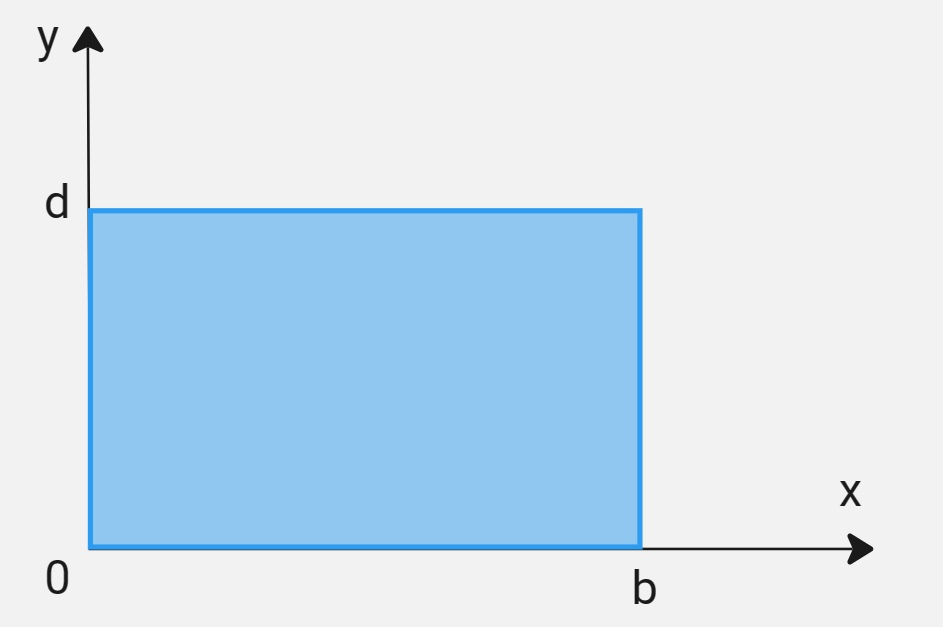
\includegraphics[width=0.5\textwidth]{p1}
		\caption{Область $\Omega$}
		\label{p1}
	 \end{figure}
	
	\subsection{Слабая постановка задачи}
	Пусть $v=v(x)$ --- гладкая функция, удовлетворяющая граничным условиям (\ref{kinem}), (\ref{silov}). Домножим на $v$ и проинтегрируем по области $\Omega$ уравнения (\ref{равновесие}):
	\begin{equation}
\begin{cases}
	\int\limits_{\Omega}v\left(	\frac{\pl\sigma_{xx}}{\pl x}+\frac{\pl\sigma_{yx}}{\pl y}+f_x\right)d\Omega=0,\\
	\int\limits_{\Omega}v\left(	\frac{\pl\sigma_{xy}}{\pl x}+\frac{\pl\sigma_{yy}}{\pl y}+f_y\right)d\Omega=0.
	\label{integrate}
\end{cases}
	\end{equation}

	Проинтегрируем первое уравнение (\ref{integrate}) по частям:
\[
	\int\limits_{\Omega}v\left(\frac{\pl\sigma_{xx}}{\pl x}+\frac{\pl\sigma_{yx}}{\pl y}+f_x\right)d\Omega=\int\limits_{\Omega}v\frac{\pl\sigma_{xx}}{\pl x}\,d\Omega+\int\limits_{\Omega}v\frac{\pl\sigma_{yx}}{\pl y}\,d\Omega+\int\limits_{\Omega}v f_{x}\,d\Omega=0.
\]
		С учетом того, что $d\Omega = dxdy,\;0\le x\le b,\;0\le y \le d$, получаем
		\begin{multline}
			\int\limits_0^d dy \int\limits_{0}^{b} v\frac{\pl\sigma_{xx}}{\pl x}\,dx+	\int\limits_0^b dx \int\limits_{0}^{d} v\frac{\pl\sigma_{yx}}{\pl y}\,dy+\int\limits_{\Omega}v f_{x}\,d\Omega=\\=\int\limits_0^d \Big(\Big. v\sigma_{xx}\Big|_0^b-\int\limits_0^b v_x\sigma_{xx}\,dx\Bigl)dy
			+\int\limits_0^b \Bigl(\Big. v\sigma_{yx}\Big|_0^d-\int\limits_0^d v_y\sigma_{yx}\,dy\Bigr)dx+\int\limits_{\Omega}v f_{x}\,d\Omega=0.
			\label{eq2}
		\end{multline}
	Подставим уравнения (\ref{Guk}) из закона Гука в (\ref{eq2}):
		\begin{multline}
%	\int_0^d \left(\Big. v\left(2\mu\varepsilon_{xx}+\lambda(\varepsilon_{xx}+\varepsilon_{yy})\right)\Big|_0^b-\int_0^b v_x\left(2\mu\varepsilon_{xx}+\lambda(\varepsilon_{xx}+\varepsilon_{yy})\right)dx\right)dy+\\
%		+\int_0^b \left(\Big. 2v\mu\varepsilon_{yx}\Big|_0^d-\int_0^d 2v_y\mu\varepsilon_{yx}dy\right)dx+\int\limits_{\Omega}v f_{x}d\Omega=0.
\int\limits_0^d \Bigl(v\left((\lambda+2\mu)(\varepsilon_{xx}-\alpha_{xx}^T\Delta T)+\lambda(\varepsilon_{yy}-\alpha_{yy}^T\Delta T)\right)\Big|_0^b-\Bigr.\\ -\Bigl.\int\limits_0^b v_x\left((\lambda+2\mu)(\varepsilon_{xx}-\alpha_{xx}^T\Delta T)+\lambda(\varepsilon_{yy}-\alpha_{yy}^T\Delta T)\right)dx\Bigr)dy+\\+\int\limits_0^b \Bigl(2\mu v(\varepsilon_{yx}-\alpha_{yx}^T\Delta T)\Big|_0^d-\int\limits_0^d 2\mu v_y(\varepsilon_{yx}-\alpha_{yx}^T\Delta T)dy\Bigr)dx+\\+\int\limits_{\Omega}v f_{x}\,d\Omega=0.
\label{eq3}
	\end{multline}

Подставим уравнения (\ref{Kochi}) в (\ref{eq3}):
\begin{multline}
%	\int_0^d \left(\Big. v\left(2\mu u_{xx}+\lambda(u_{xx}+u_{yy})\right)\Big|_0^b-\int_0^b v_x\left(2\mu u_{xx}+\lambda(u_{xx}+u_{yy})\right)dx\right)dy+\\
%	+\int_0^b \left(\Big. v\mu(u_{xy}+u_{yx})\Big|_0^d-\int_0^dv_y\mu(u_{xy}+u_{yx})dy\right)dx+\int\limits_{\Omega}v f_{x}d\Omega=0.
	\int\limits_0^d \left(v\left((\lambda+2\mu)\left(\frac{\pl u_x}{\pl x}-\alpha_{xx}^T\Delta T\right)+\lambda\left(\frac{\pl u_y}{\pl y}-\alpha_{yy}^T\Delta T\right)\right)\Big|_0^b-\right.\\ -\left.\int\limits_0^b v_x\left((\lambda+2\mu)\left(\frac{\pl u_x}{\pl x}-\alpha_{xx}^T\Delta T\right)+\lambda\left(\frac{\pl u_y}{\pl y}-\alpha_{yy}^T\Delta T\right)\right)dx\right)dy+\\
	+\int\limits_0^b \left(\mu v\left(\left(\frac{\pl u_x}{\pl y}+\frac{\pl u_y}{\pl x}\right)-\alpha_{yx}^T\Delta T\right)\Big|_0^d-\int\limits_0^d \mu v_y\left(\left(\frac{\pl u_x}{\pl y}+\frac{\pl u_y}{\pl x}\right)-\alpha_{yx}^T\Delta T\right)dy\right)dx+\\+\int\limits_{\Omega}v f_{x}\,d\Omega=0.
		\label{eq4}
\end{multline}

Таким образом, от исходной задачи (\ref{Kochi})--(\ref{silov}) приходим к слабой постановке задачи: определить $u\in V$, такое, что

\[\begin{gathered}
\int\limits_\Omega\varepsilon(v):\mathbb C:\varepsilon(u)\,d\Omega=\int\limits_\Omega f v\, d\Omega+\int\limits_{\Gamma_N} p v \,dS,\quad v\in V_D,\\
Mu=w \text{ на } \Gamma_D,
\end{gathered}
\]
где $V$ --- пространство достаточно гладких векторных полей, а пространство $V_D$ определено как
\[
V_D=\{v\in V:Mv=0\text{ на } \Gamma_D\}.
\]

Аппроксимируем приведенную задачу методом Галеркина \cite{galanin1}.
\newpage
\subsection{Метод конечных элементов}
Представим расчетную область $\Omega$ в виде объединения треугольных подобластей $\Omega = \sum\limits_{p=1}^N \Omega_p,\,N$ --- количество элементов, т.е. построим \textit{триангуляцию} области $\Omega$. 

Выберем пространство пробных функций, состоящее	из финитных функций $\phi_{pm},\,\\p=1,\dots,N,\,m=1,2,3.$ Будем аппроксимировать поле перемещений функциями из данного пространства. Представим решение в следующем виде:
\begin{equation}
	\begin{cases}
		u_x=\sum\limits_{p=1}^N\sum\limits_{m=1}^3 u_{pm}^{(x)}\phi_{pm},\\
		u_y=\sum\limits_{p=1}^N\sum\limits_{m=1}^3 u_{pm}^{(y)}\phi_{pm},
		\label{ishemvvide}	
	\end{cases}
\end{equation}
 где $u_p^{(x)},\,u_p^{(y)}$ --- неизвестные весовые коэффициенты.

В качестве финитных функций (функций формы) выберем следующие:
\[
\phi_{pm} = 
\begin{cases}
	N_{pm}=\frac{1}{\Delta}\left(a_{pm}+b_{pm} x+c_{pm} y\right),\\
	a_{pm}=x_{qm}y_{rm}-x_{rm}y_{qm},\\
	b_{pm}=y_{qm}-y_{rm},\\
	c_{pm}=x_{rm}-x_{qm},\\
	\Delta=(x_{qm}-x_p)(y_{rm}-y_p)-(x_{rm}-x_p)(y_{qm}-y_p).\\
\end{cases}
\]

Подставив (\ref{ishemvvide}) в (\ref{eq4}) получаем
% Просто подставили
%\begin{multline}
%	\int\limits_0^d \Bigl(v\left((\lambda+2\mu)\left(u_p^{(x)}\frac{\pl \phi_p}{\pl x}-\alpha_{xx}^T\Delta T\right)+\lambda\left(u_p^{(y)}\frac{\pl \phi_p}{\pl y}-\alpha_{yy}^T\Delta T\right)\right)\Big|_0^b-\Bigr.\\ -\Bigl.\int\limits_0^b v_x\left((\lambda+2\mu)\left(u_p^{(x)}\frac{\pl \phi_p}{\pl x}-\alpha_{xx}^T\Delta T\right)+\lambda\left(u_p^{(y)}\frac{\pl \phi_p}{\pl y}-\alpha_{yy}^T\Delta T\right)\right)dx\Bigr)dy+\\
%	+\int\limits_0^b \left(\mu v\left(\left( u_p^{(x)}\frac{\pl \phi_p}{\pl y}+ u_p^{(y)}\frac{\pl \phi_p}{\pl x}\right)-\alpha_{yx}^T\Delta T\right)\Big|_0^d-\int\limits_0^d \mu v_y\left(\left(u_p^{(x)}\frac{\pl \phi_p}{\pl y}+ u_p^{(y)}\frac{\pl \phi_p}{\pl x}\right)-\alpha_{yx}^T\Delta T\right)dy\right)dx+\\+\int\limits_{\Omega}v f_{x}d\Omega=0.
%	\label{eq5}
%\end{multline}

%Слева оператор, справа известная часть
\begin{multline}
	\int\limits_0^d\int\limits_0^b \left(\frac{\pl \phi_m}{\pl x}(\lambda+2\mu)\left(u_p^{(x)}\frac{\pl \phi_p}{\pl x}-\alpha_{xx}^T\Delta T\right)+\frac{\pl \phi_m}{\pl x}\lambda\left(u_p^{(y)}\frac{\pl \phi_p}{\pl y}-\alpha_{yy}^T\Delta T\right)\right.+\\ \left.
	\mu \frac{\pl \phi_m}{\pl y}\left(u_p^{(x)}\frac{\pl \phi_p}{\pl y}+ u_p^{(y)}\frac{\pl \phi_p}{\pl x}\right)-\mu \frac{\pl \phi_m}{\pl y}\alpha_{yx}^T\Delta T\right)dxdy=\\
	=\int\limits_0^d \left(\phi_m(\lambda+2\mu)\left(u_p^{(x)}\frac{\pl \phi_p}{\pl x}-\alpha_{xx}^T\Delta T\right)+\phi_m\lambda\left(u_p^{(y)}\frac{\pl \phi_p}{\pl y}-\alpha_{yy}^T\Delta T\right)\right)\Big|_0^b dy+\\
	+\int\limits_0^b \left(\mu \phi_m\left( u_p^{(x)}\frac{\pl \phi_p}{\pl y}+ u_p^{(y)}\frac{\pl \phi_p}{\pl x}\right)-\mu \phi_m\alpha_{yx}^T\Delta T\right)\Big|_0^d dx	+\int\limits_{\Omega}\phi_m f_{x}\,d\Omega.
	\label{equilib1}
\end{multline}

Аналогично получаем для второго уравнения равновесия (\ref{integrate})
%\[
%	\int\limits_{\Omega}v\left(	\frac{\pl\sigma_{xy}}{\pl x}+\frac{\pl\sigma_{yy}}{\pl y}+f_y\right)d\Omega=0.
%\]
%\[
%	\int\limits_{\Omega}v\left(	\frac{\pl\sigma_{xy}}{\pl x}+\frac{\pl\sigma_{yy}}{\pl y}+f_y\right)d\Omega=\int\limits_{\Omega}v\frac{\pl\sigma_{xy}}{\pl x}d\Omega+\int\limits_{\Omega}v\frac{\pl\sigma_{yy}}{\pl y}d\Omega+\int\limits_{\Omega}v f_{y}d\Omega=0.
%\]
%	С учетом того, что $d\Omega = dxdy,\;0\le x\le b,\;0\le y \le d$, получаем
%\begin{multline}
%	\int\limits_0^d dy \int\limits_{0}^{b} v\frac{\pl\sigma_{xy}}{\pl x}dx+	\int\limits_0^b dx \int\limits_{0}^{d} v\frac{\pl\sigma_{yy}}{\pl y}dy+\int\limits_{\Omega}v f_{y}d\Omega=\\=\int\limits_0^d \Big(\Big. v\sigma_{xy}\Big|_0^b-\int\limits_0^b v_x\sigma_{xy}dx\Bigl)dy
%	+\int\limits_0^b \Bigl(\Big. v\sigma_{yy}\Big|_0^d-\int\limits_0^d v_y\sigma_{yy}dy\Bigr)dx+\int\limits_{\Omega}v f_{y}d\Omega=0.
%\end{multline}
%	Подставим уравнения (\ref{Guk}) из закона Гука в (\ref{eq2}):
%\begin{multline}
%\int\limits_0^d \Big(\Big. 2v\mu(\varepsilon_{xy}-\alpha_{xy}^T\Delta T)\Big|_0^b-\int\limits_0^b 2v_x\mu(\varepsilon_{xy}-\alpha_{xy}^T\Delta T)dx\Bigl)dy
%	+\\+\int\limits_0^b \Bigl(\Big. v\left(\lambda(\varepsilon_{xx}-\alpha_{xx}^T\Delta T)+(\lambda+2\mu)(\varepsilon_{yy}-\alpha_{yy}^T\Delta T)\right)\Big|_0^d-\\-\int\limits_0^d v_y\left(\lambda(\varepsilon_{xx}-\alpha_{xx}^T\Delta T)+(\lambda+2\mu)(\varepsilon_{yy}-\alpha_{yy}^T\Delta T)\right)dy\Bigr)dx+\int\limits_{\Omega}v f_{y}d\Omega=0.
%\end{multline}
%\begin{multline}
%	\int\limits_0^d \Big(\Big. 2v\mu(\frac12 \left(\frac{\pl u_x}{\pl y}+\frac{\pl u_y}{\pl x}\right)-\alpha_{xy}^T\Delta T)\Big|_0^b-\int\limits_0^b 2v_x\mu(\frac12 \left(\frac{\pl u_x}{\pl y}+\frac{\pl u_y}{\pl x}\right)-\alpha_{xy}^T\Delta T)dx\Big)dy
%	+\\+\int\limits_0^b \Bigl(\Big. v\left(\lambda(\frac{\pl u_x}{\pl x}-\alpha_{xx}^T\Delta T)+(\lambda+2\mu)(\frac{\pl u_y}{\pl y}-\alpha_{yy}^T\Delta T)\right)\Big|_0^d-\\-\int\limits_0^d v_y\left(\lambda(\frac{\pl u_x}{\pl x}-\alpha_{xx}^T\Delta T)+(\lambda+2\mu)(\frac{\pl u_y}{\pl y}-\alpha_{yy}^T\Delta T)\right)dy\Bigr)dx+\int\limits_{\Omega}v f_{y}d\Omega=0.
%\end{multline}
\begin{multline}
\int\limits_0^d \int\limits_0^b \left(\frac{\pl \phi_m}{\pl x}\mu\left( u_p^{(x)}\frac{\pl \phi_p}{\pl y}+ u_p^{(y)}\frac{\pl \phi_p}{\pl x}\right)-2\frac{\pl \phi_m}{\pl x}\mu\alpha_{xy}^T\Delta T+\right.\\ \left.+\lambda\frac{\pl \phi_m}{\pl y}\left(u_p^{(x)}\frac{\pl \phi_p}{\pl x}-\alpha_{xx}^T\Delta T\right)+\frac{\pl \phi_m}{\pl y}(\lambda+2\mu)\left(u_p^{(y)}\frac{\pl \phi_p}{\pl y}-\alpha_{yy}^T\Delta T\right)\right)dydx=\\=	\int\limits_0^d \left(\phi_m\mu \left( u_p^{(x)}\frac{\pl \phi_p}{\pl y}+ u_p^{(y)}\frac{\pl \phi_p}{\pl x}\right)-2\phi_m\mu\alpha_{xy}^T\Delta T\right)\Big|_0^b dy+\\+\int\limits_0^b \left(\phi_m\lambda\left(u_p^{(x)}\frac{\pl \phi_p}{\pl x}-\alpha_{xx}^T\Delta T\right)+\phi_m(\lambda+2\mu)\left(u_p^{(y)}\frac{\pl \phi_p}{\pl y}-\alpha_{yy}^T\Delta T\right)\right)\Big|_0^d dx+\int\limits_{\Omega}\phi_m f_{y}\,d\Omega.
\label{equilib2}
\end{multline}

Уравнения (\ref{equilib1}) и (\ref{equilib2}) приведены к виду
\[
\sum\limits_{p=1}^{N}\left(\int\limits_\Omega\varepsilon(\phi_m):\mathbb{C}:\varepsilon(\phi_p)\,d\Omega\right)u_p=\int\limits_\Omega f\phi_m\,d\Omega+\int\limits_{\Gamma_N}p\phi_m \,dS,
\]
или в матричном виде $Au_h=F$, где
\[
A_{pm} = \int\limits_\Omega \varepsilon(\phi_m):\mathbb{C}:\varepsilon(\phi_p)\, d\Omega,\quad F_m=\int\limits_\Omega f \phi_m\,d\Omega+\int\limits_{\Gamma_N}p\phi_m\,dS,\quad m,\,p=\overline{1,N}.
\]
\section{Тестовый расчет}
\subsection{Исходные данные}
Возьмем область (пластинку) с параметрами $b = 8$ мм, $d = 8$ мм. Для численного анализа метода конечных элементов (МКЭ) зададим произвольное аналитическое решение задачи $u(x,y)$ и найдем из уравнений ($\ref{Kochi}),\,(\ref{Guk})$ и ($\ref{равновесие}$) плотности массовых сил $f_x,\,f_y$.

Физические характеристики диоксида урана UO$_2$: 
\begin{itemize}
%	\item предел прочности $\sigma_f = 1,1\cdot 10^8$ Па;
%	\item предел деформации $\varepsilon_f=0.000628571$;
	\item модуль Юнга $E = 1,75\cdot 10^{11}$ Па;
	\item коэффициент Пуассона $\nu = 0,316$;
	\item плотность $\rho=10800$ кг/м$^3$;
	\item удельная теплоемкость $c_\varepsilon=310$ Дж/(кг$\cdot$К);
	\item теплопроводность $\lambda=3,487$ Вт/(м$\cdot$К);
	\item предел прочности напряжений $\sigma_f = 1,1\cdot10^8$ Па;
	\item коэффициент теплового расширения $\alpha = 10^{-5}\text{ K}^{-1}$;
	\item температура естественного состояния $T_{ref} = 300$ К.
	\end{itemize}
\subsection{Численный анализ}
%\paragraph{Пример 1}
%	 Найдем порядок сходимости задачи без распределения температуры: 
%	 
%\[
%\textbf{u} =(xy;xy)\text{ --- точное решение},\quad f_x =f_y= \frac{E}{4\nu^2+2\nu-2}.\]
%Возьмем сетку следующего типа:
%	\begin{figure}[H]
%	\centering
%	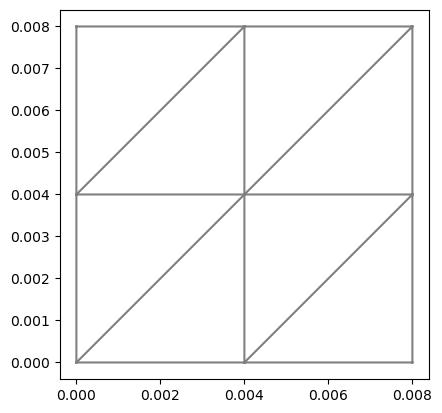
\includegraphics[width=0.3\linewidth]{grid}
%	\caption{Структурированная равномерная сетка}
%\end{figure}
%\[
%T(x,y) = \sqrt{\left(x-\frac{b}{2}\right)^2+\left(y-\frac{d}{2}\right)^2},\quad (x,y)\in \Omega.
%\]
	\begin{figure}[H]
	\centering
	\begin{subfigure}[H]{0.4\textwidth}
		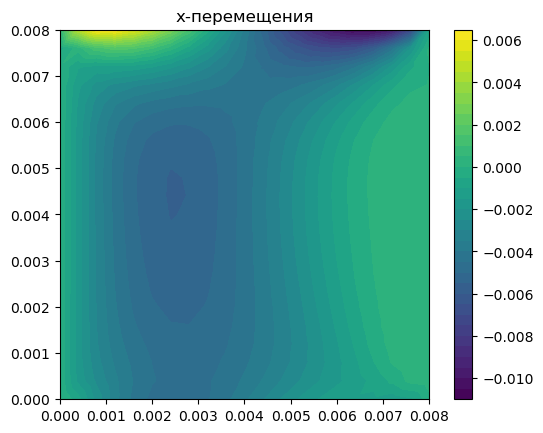
\includegraphics[width=\textwidth]{x0}
	\end{subfigure}
	\qquad\qquad
	\begin{subfigure}[H]{0.4\textwidth}
		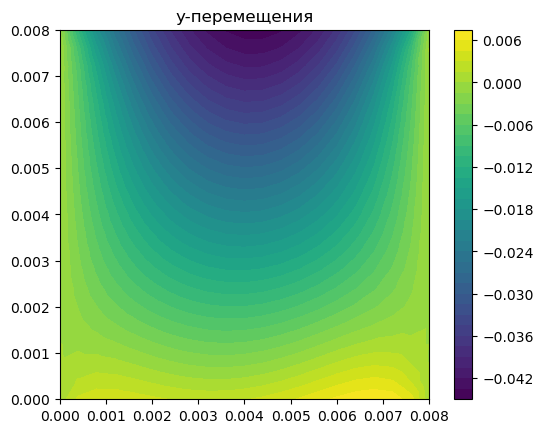
\includegraphics[width=\textwidth]{y0}
	\end{subfigure}	
	\\[0.2cm]
	\caption{Перемещения}
	\begin{subfigure}[H]{0.4\textwidth}
		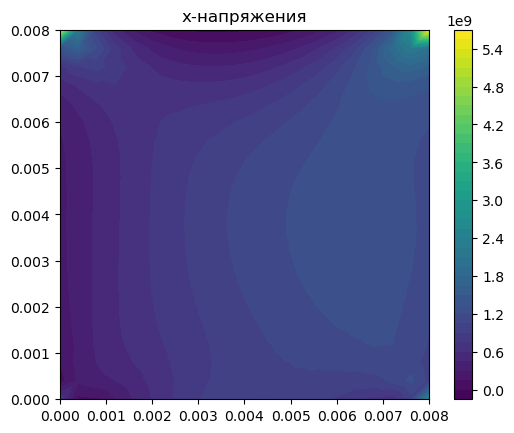
\includegraphics[width=\textwidth]{stress0}
	\end{subfigure}
	\qquad\qquad
	\begin{subfigure}[H]{0.4\textwidth}
		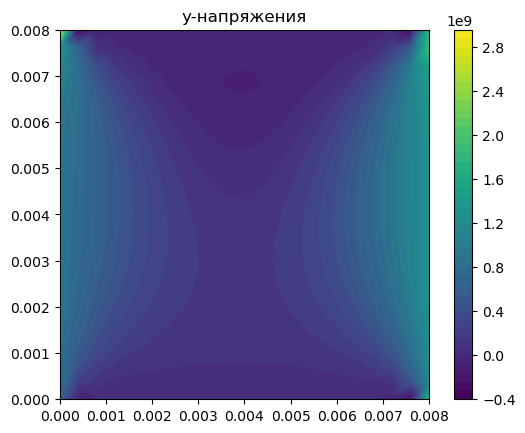
\includegraphics[width=\textwidth]{stressy0}
	\end{subfigure}	
	\\[0.2cm]
	\caption{Напряжения}
\end{figure}	
\begin{table}[H]
\caption{Порядок сходимости}
\centering
\footnotesize
\begin{tabular}{|c|c|c|c|c|}
	\hline
	Параметры сетки & AbsErr$_{C}$ & $\Delta_C$ & AbsErr$_{L_2}$ & $\Delta_{L_2}$ \\ 
	\hline
	\multicolumn{5}{|c|}{$\mathbf{u} = \left(xy\,;\,xy\right),\quad T(x,y) = x^2+y^2$}\\
	\hline
	\makecell{Количество узлов: 9\\
	 Количество элементов: 8\\ Количество граничных узлов: 8} &1.918e-06&&8.750e-07&\\
		\hline
	\makecell{Количество узлов: 25\\ Количество элементов: 32\\ Количество граничных узлов: 16} &2.979e-07&6.4384&1.878e-07&4.6592\\
		\hline
	\makecell{Количество узлов: 81\\ Количество элементов: 128\\ Количество граничных узлов: 32 } &7.7783e-08&3.8300&3.7796e-08&4.6695\\
		\hline
	\makecell{Количество узлов: 289\\ Количество элементов: 512\\ Количество граничных узлов: 64 } &1.981e-08&3.9106&1,0510e-08 &3.5956\\
		\hline
	
	\end{tabular}
\end{table}
В таблице приведены ошибки в нормах $\|.\|_C$ и $\|.\|_{L_2}$, AbsErr --- абсолютная ошибка, $\Delta$ --- модуль отношения ошибок на двух соседних сетках.
\newpage
В качестве функции температуры возьмем:
\[
T(x,y) = -1000\sqrt{\left(x-\frac{b}{2}\right)^2+\left(y-\frac{d}{2}\right)^2}
\]
\begin{table}[H]
	\caption{Порядок сходимости}
	\centering
	\footnotesize
	\begin{tabular}{|c|c|c|c|c|}
		\hline
		Параметры сетки & AbsErr$_{C}$ & $\Delta_C$ & AbsErr$_{L_2}$ & $\Delta_{L_2}$ \\ 
		\hline
		\multicolumn{5}{|c|}{$\mathbf{u} = \left(e^{x^2+y^2}\,;\,\tanh(xy)\right)$}\\
		\hline
		\makecell{Количество узлов: 5\\
			Количество элементов: 4\\ Количество граничных узлов: 4} &1.9320e-06&&8.6403e-07&\\
		\hline
		\makecell{Количество узлов: 12\\ Количество элементов: 14\\ Количество граничных узлов: 8} &2.8491e-07&6.7812&1.4671e-07&5.8893\\
		\hline
		\makecell{Количество узлов: 36\\ Количество элементов: 54\\ Количество граничных узлов: 16 } &7.7783e-08&3.6629&3.7796e-08&3.88172\\
		\hline
		\makecell{Количество узлов: 136\\ Количество элементов: 238\\ Количество граничных узлов: 32 } &2.0339e-08& 3.8244&1.0721e-08 &3.5255\\
		\hline
		\makecell{Количество узлов: 509\\ Количество элементов: 952\\ Количество граничных узлов: 64 } &6.3894e-09&3.6139&3.2510e-09 &3.6250\\
		\hline
		\multicolumn{5}{|c|}{$\mathbf{u} = \left(y^2e^x\,;\,\cos(xy)+\sin(xy)\right)$}\\
		\hline
		\makecell{Количество узлов: 5\\
			Количество элементов: 4\\ Количество граничных узлов: 4} &2.0485e-06&&9.1612e-07&\\
		\hline
		\makecell{Количество узлов: 12\\ Количество элементов: 14\\ Количество граничных узлов: 8} &3.2178e-07&6.3660&1.8426e-07&4.9718\\
		\hline
		\makecell{Количество узлов: 36\\ Количество элементов: 54\\ Количество граничных узлов: 16 } &9.9139e-08&3.2458&4.9698e-08&3.7077\\
		\hline
		\makecell{Количество узлов: 136\\ Количество элементов: 238\\ Количество граничных узлов: 32 } &2.3091e-08&4.2934&1.1785e-08 &4.2170\\
		\hline
		\makecell{Количество узлов: 509\\ Количество элементов: 952\\ Количество граничных узлов: 64 } &6.3894e-09&3.6139&3.2510e-09 &3.6320\\
		\hline
	\end{tabular}
\end{table}

В качестве конечных элементов выбраны стандартные линейные лагранжевы элементы. Из результатов видно, что сходимость схемы со вторым порядком точности.
\subsection{Линейная (несвязная) термоупругая задача}
В качестве постановки задачи для термоупругости также можно добавить уравнение теплопроводности без \textit{термомеханической связности} для изотропного тела:
\[
\rho c_\varepsilon\frac{\pl T}{\pl t} =\frac{\pl}{\pl x_i}\left(\lambda_{ij}\frac{\pl T}{\pl x_j}\right)+f\quad \Leftrightarrow\quad \rho c_\varepsilon\frac{\pl T}{\pl t}=\mathrm{div}(\lambda\,\mathrm{grad}\, T)+f,
\]
Для стационарного случая получим эллиптическое уравнение
\begin{equation}
-\mathrm{div}(\lambda\,\mathrm{grad}\, T)=f
\label{sta}
\end{equation}
В постоянном режиме температурное поле отделено от механических полей, а последние зависят от температуры из-за наличия тепловых деформаций.
\bigskip

Рассмотрим стационарный режим и положим $f=0$. Пусть верхняя и нижняя стороны пластинки находится по температурой $T_{ref}$, а боковые стороны зажаты и их нагревают на $\Delta T=100$ К.
 	\begin{figure}[H]
	\centering
	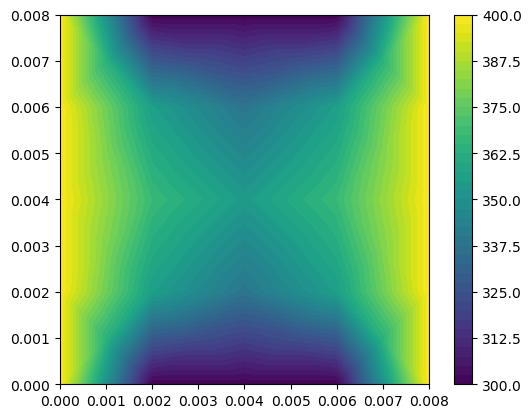
\includegraphics[width=0.4\textwidth]{tempreture1}
	\caption{Температурное поле}
\end{figure}
	\begin{figure}[H]
		\centering
		\begin{subfigure}[H]{0.4\textwidth}
			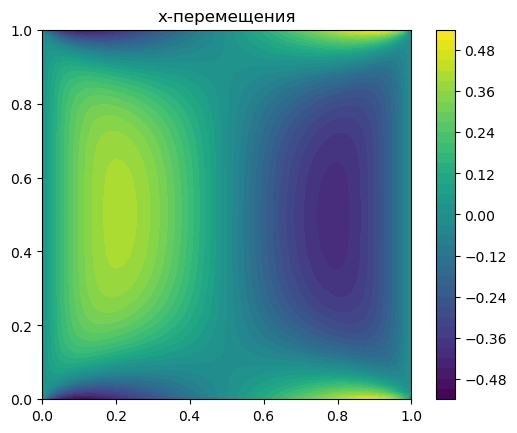
\includegraphics[width=\textwidth]{horiz1}
		\end{subfigure}
		\qquad\qquad
		\begin{subfigure}[H]{0.4\textwidth}
			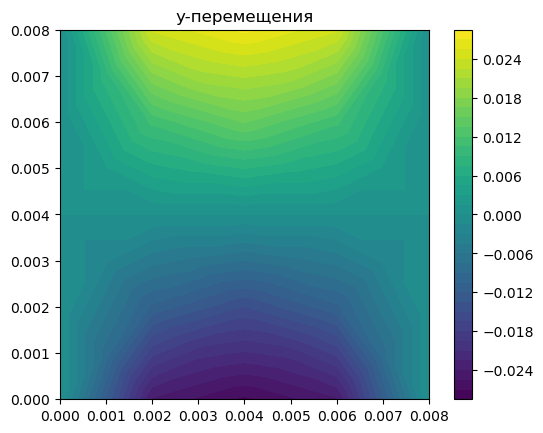
\includegraphics[width=\textwidth]{vert1}
		\end{subfigure}	
		\\[0.2cm]
		\caption{Перемещения}
	\end{figure}	
	\begin{figure}[H]
	\centering
	\begin{subfigure}[H]{0.4\textwidth}
		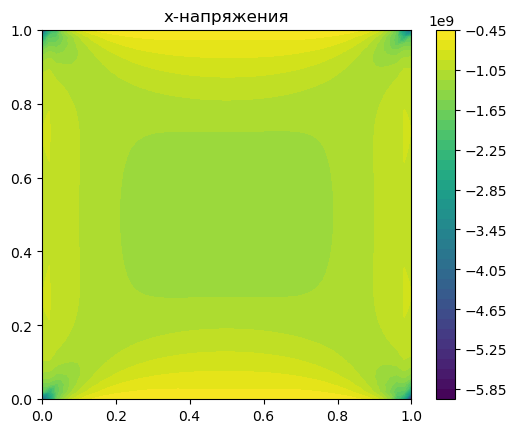
\includegraphics[width=\textwidth]{stress_x}
	\end{subfigure}
	\qquad\qquad
	\begin{subfigure}[H]{0.4\textwidth}
		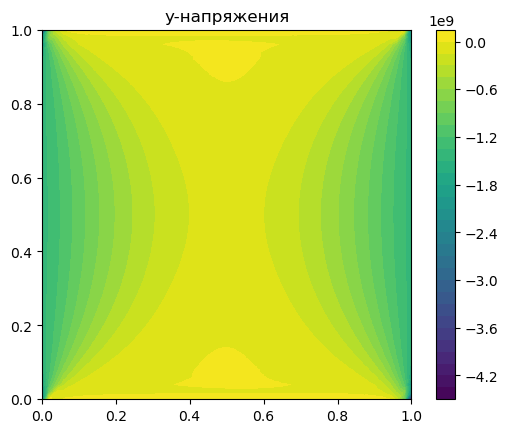
\includegraphics[width=\textwidth]{xtress_y}
	\end{subfigure}	
	\\[0.2cm]
	\caption{Напряжения}
\end{figure}	

Рассмотрим нестационарную задачу и положим $f=0$.
\[
\rho c_\varepsilon\frac{\pl T}{\pl t}=\mathrm{div}(\lambda\,\mathrm{grad}\, T),
\]
 Для дискретизации по времени воспользуемся методом конечных разностей. Временной интервал разобъем на $M+1$ слоев с шагом $\tau = \sfrac{T_f}{M}$. На каждом из них будем решать стационарную задачу теории упругости с учетом температуры.
 
Параметры задачи:
\[
\begin{gathered}
	T(x,y,0) =T_{ref},\\ T(0,y,t)=T(b,y,t) = T_{ref},\\ T(x,0,t)=T(x,d,t)=400 \text{ К},\\
	u(0,y,t)=u(d,0,t)=0,\\
	T_f = 10 \text{ c},\; M = 10. 
\end{gathered}
\]
	\begin{figure}[H]
	\centering
	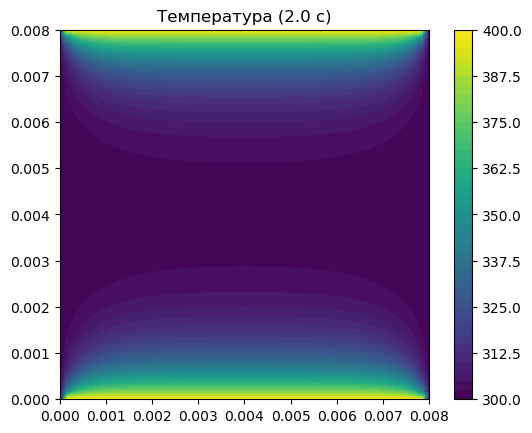
\includegraphics[width=0.45\textwidth]{temp_2c}
	\caption{Температурное поле}
\end{figure}
\begin{figure}[H]
	\centering
	\begin{subfigure}[H]{0.38\textwidth}
		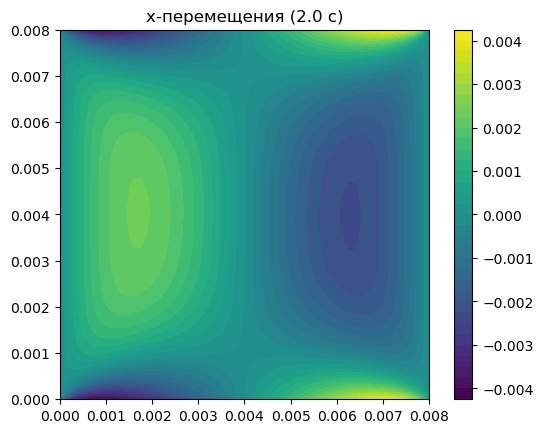
\includegraphics[width=\textwidth]{ux_2c}
	\end{subfigure}
	\qquad\qquad
	\begin{subfigure}[H]{0.38\textwidth}
		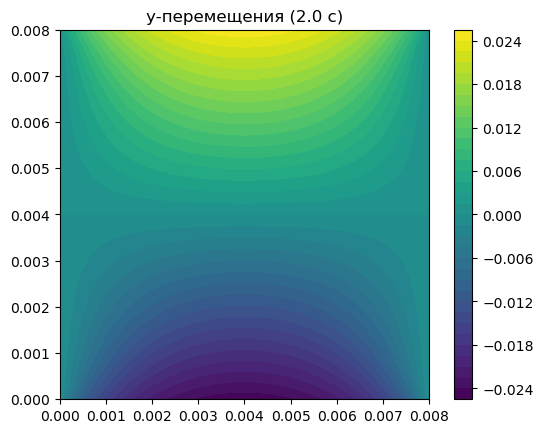
\includegraphics[width=\textwidth]{uy_2c}
	\end{subfigure}	
	\\[0.2cm]
	\caption{Перемещения}
\end{figure}	
\begin{figure}[H]
	\centering
	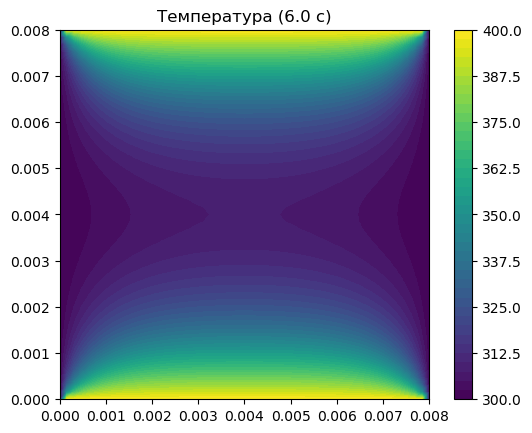
\includegraphics[width=0.38\textwidth]{temp_6c}
	\caption{Температурное поле}
	\centering
	\begin{subfigure}[H]{0.38\textwidth}
		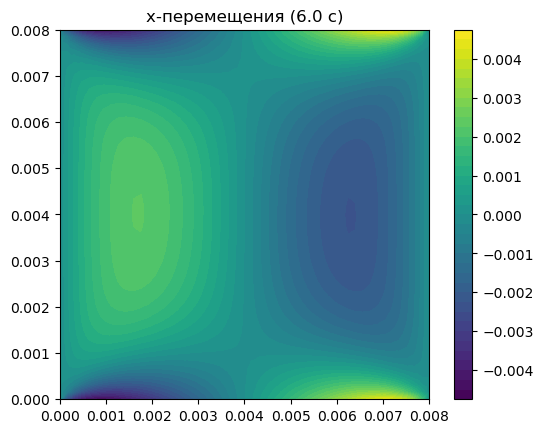
\includegraphics[width=\textwidth]{ux_6c}
	\end{subfigure}
	\qquad\qquad
	\begin{subfigure}[H]{0.38\textwidth}
		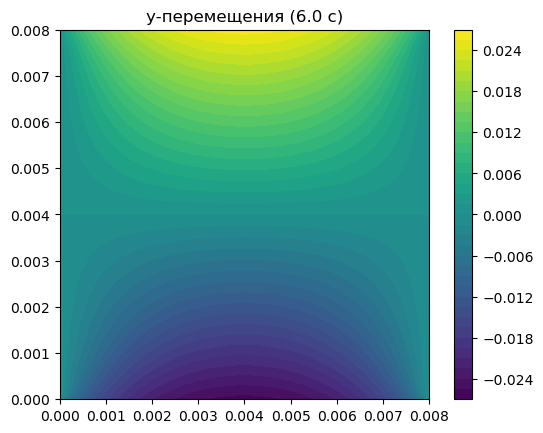
\includegraphics[width=\textwidth]{uy_6c}
	\end{subfigure}	
	\\[0.2cm]
	\caption{Перемещения}
	\begin{subfigure}[H]{0.38\textwidth}
		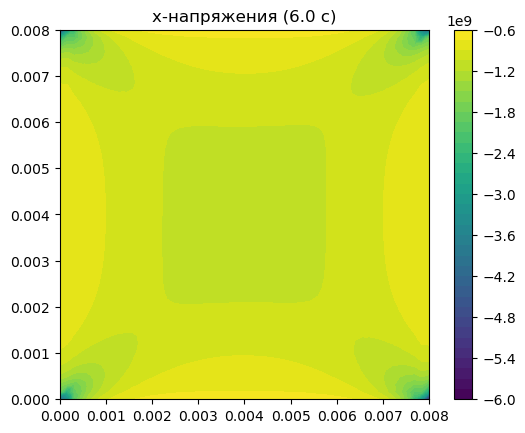
\includegraphics[width=\textwidth]{stressx_6c}
	\end{subfigure}
	\qquad\qquad
	\begin{subfigure}[H]{0.38\textwidth}
		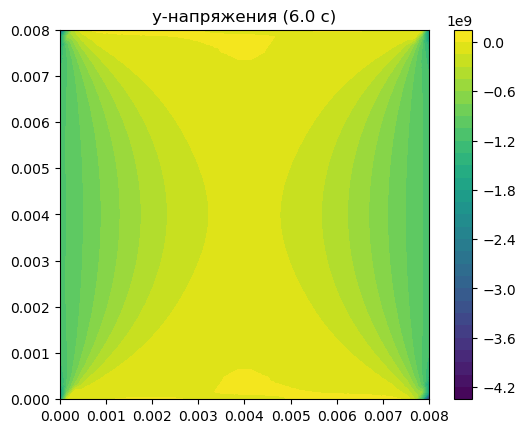
\includegraphics[width=\textwidth]{stressy_6c}
	\end{subfigure}	
	\\[0.2cm]
	\caption{Напряжения}
\end{figure}	
 
\newpage
\section{Разрушение топливных таблеток}
\subsection{Модель размазанных трещин}
Для моделирования разрушения топливных таблеток из диоксида урана (UO$_2$) применяют подход размазанных трещин \cite{galanin1}.
\begin{figure}[H]
	\centering
	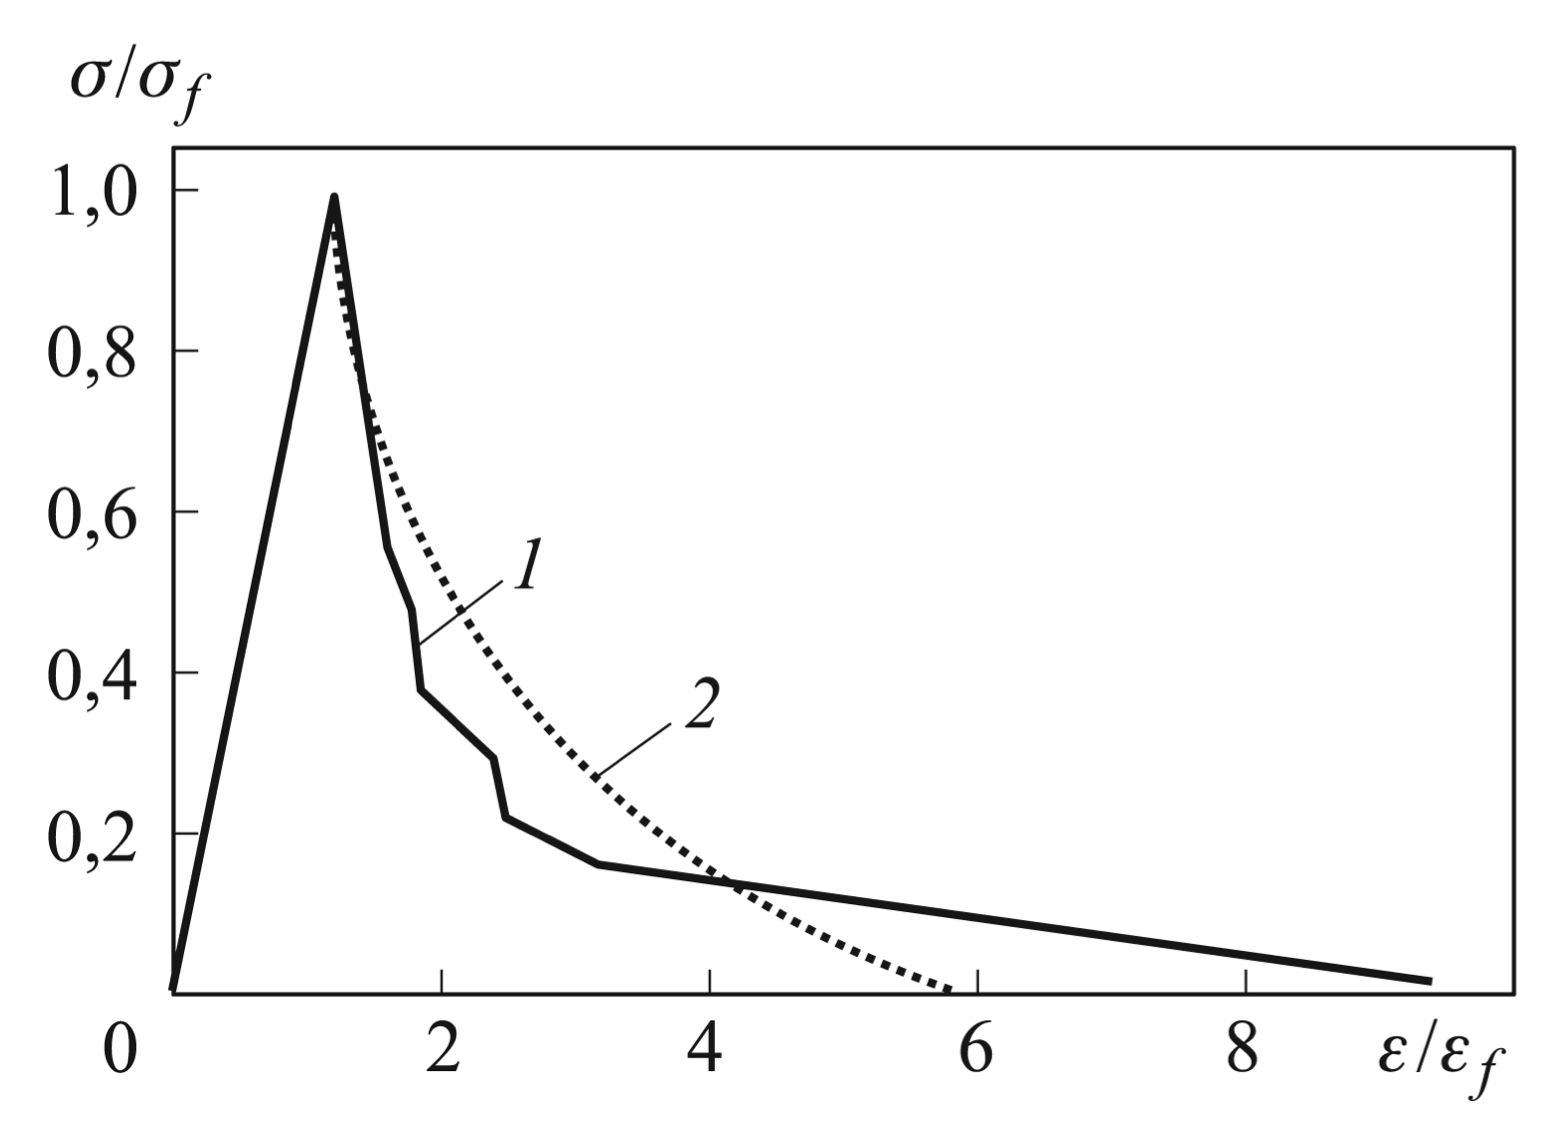
\includegraphics[width=0.5\textwidth]{ceramic}
	\caption{Экспериментальная (1) и аналитическая (2) кривые нормализованного растягивающего отклика для керамических материалов}
	\label{fig:ceramic}
\end{figure}
На рис. \ref{fig:ceramic} видно, что пока напряжение меньше предела прочности $\sigma < \sigma_f$  и деформации меньше соответствующего значения $\varepsilon < \varepsilon_f$, материал ведет себя, как линейно-упругий, а затем происходит разгрузка по нелинейному закону. При достижении предельного значения прочности $\sigma_f$ происходит инициализация трещины. Она формируется лишь после достижения значений деформаций, превышающих $\varepsilon_f$ в $5-10$ раз. Кривую, имеющую данный характер поведения, можно аппроксимировать в следующем виде:
\begin{equation}
\dfrac{\sigma}{\sigma_f} = A + B e^{-C\tfrac{\varepsilon}{\varepsilon_f}},
\label{ceramic}
\end{equation}
\noindent где $A \approx -0.024, B \approx 1.69, C \approx 0.5$. Полагается, что зависимость (\ref{ceramic}) справедлива при $\varepsilon<\varepsilon_0$ ($\varepsilon_0$ --- значение деформации, большее предела прочности в 5-10 раз, при котором материал не передает напряжения в направлении, ортогональном направлению трещины).
\subsection{Математическая модель}
Будем рассматривать две конфигурации твердого тела --- без растрескивания (\textit{K$_1$}) и с учетом образования трещин (\textit{K$_2$}). Для начала определим некоторые соотношения.

Зависимость (\ref{ceramic}) запишем в другом виде
\[
\begin{gathered}
\frac{\sigma}{\sigma_f}=\frac{\sigma}{\varepsilon} \frac{\varepsilon}{\varepsilon_f}\frac{\varepsilon_f}{\sigma_f}=A+Be^{-C\sfrac{\varepsilon}{\varepsilon_f}},\\
E=\frac{\sigma}{\varepsilon},\quad E_0=\frac{\sigma_f}{\varepsilon_f} \Rightarrow \frac{E}{E_0}\frac{\varepsilon}{\varepsilon_f}=A+Be^{-C\sfrac{\varepsilon}{\varepsilon_f}},
\end{gathered}
\]
где $E$ и $E_0$ --- текущий и начальный модули Юнга.

Тогда введем функцию памяти материала $e(t)$ для двумерного случая:
\begin{equation}
	e_i(t) =
	\begin{cases}
		0,\quad \varepsilon_i>\varepsilon_0,\\
\sfrac{E}{E_0}=\sfrac{\varepsilon_f}{\varepsilon_i}\left(A+Be^{-C\sfrac{\varepsilon}{\varepsilon_f}}\right),\quad \varepsilon_f\le\varepsilon_i\le\varepsilon_0,\\
1,\quad \varepsilon_i<\varepsilon_f,\\
i=1,2.
	\end{cases}	
\end{equation}
Для двумерной задачи определим матрицу $\hat E$
\[
\hat{E}=
\begin{pmatrix}
	e_1&0&0\\
	0&e_2&0\\
	0&0&e_1e_2
\end{pmatrix},
\]
которая является матрицей перехода: $K_1 \rightarrow K_2$.

Для того, чтобы использовать функцию памяти необходимо привести тензор деформации $\hat\varepsilon$ к главным осям. Введем матрицу перехода $\hat T$, которая диагонализирует тензор деформаций $\hat \varepsilon$
\[
\begin{pmatrix}
\varepsilon_1&0\\
0&\varepsilon_2
\end{pmatrix}=
\hat{T}^{-1}\,\hat{\varepsilon} \hat T.
\]
Известно, что из матрицы $\hat T$ единственным образом составляется матрица преобразования $\hat P$, которая приводит вектор деформаций $\vec \varepsilon$ в нотации Фойгта к следующему виду $\overline{\varepsilon}=\{\varepsilon_1,\varepsilon_2,0\}^{\mathrm T}$\footnote{Символ $\,\overline{\,\,\cdotp\,\,}\,$ обозначает запись в главных осях.}.

 Для конфигурации \textit{K$_1$} справедлив закон Гука:
\[
\vec \sigma = [C]\,\vec{\varepsilon^e}.
\]

Рассмотрим в конфигурации \textit{K$_1$} систему координат, связанную главными направлениями тензора деформаций. В этой системе координат закон Гука имеет вид
\[
\overline{\sigma}=[\overline{C}]\,\overline{\varepsilon}^e.
\]
Отметим, что матрица перехода $\hat{P}$ к главным направлениям тензора деформаций является ортогональной, поэтому
\[
\vec{\varepsilon}^T\,\vec \sigma=\overline{\varepsilon}^T\,\overline{\sigma}.
\]
Закон Гука для конфигурации $K_2$ имеет вид
\[
\tilde{\sigma}=\tilde{C}\left(\tilde{\varepsilon}-\tilde{\varepsilon}^T\right).
\label{K2}
\] 
Поскольку матрица перехода $\hat{E}$ из конфигурации $K_1$ в конфигурацию $K_2$ является диагональной и поворота осей при этом не происходит, то соотношение (\ref{K2}) будет иметь вид 
\[
\overline{\sigma}=\tilde{C}\left(\overline{\varepsilon}-\overline{\varepsilon}^T\right),\quad \tilde{C}=\hat E^T\,\overline{C}\,\hat E.
\] 

Вернемся к исходной системе координат с помощью соотношений
\[
\begin{gathered}
\vec\sigma = \hat P^{\mathrm T}\,\overline{\sigma},\quad \vec \varepsilon=\hat P^{-1} \overline{\varepsilon},\quad \overline{C}=\left(\hat P^{-1}\right)^{\mathrm T}\,[C]\,\hat P^{-1},\\
\Rightarrow \vec \sigma =  \hat P^{\mathrm T}\tilde C \hat P\left(\vec \varepsilon-\vec \varepsilon^T\right).
\end{gathered}
\]
причем
\[
\begin{gathered}
\hat P^{\mathrm T}\tilde C \hat P = \hat P^{\mathrm T}\hat E^T\,\overline{C}\,\hat E \hat P=\left(\hat P^{\mathrm T}\hat E^T(\hat P^{-1})^{\mathrm T}\right)[C]\left(\hat P^{-1}\hat E \hat P\right),\\
\hat Z=\hat P^{-1}\hat E \hat P.
\end{gathered}
\]
Тогда 
\[
\vec \sigma =  \hat Z^{\mathrm T} \hat C \hat Z\left(\vec \varepsilon-\vec \varepsilon^T\right) = \hat C^{\mathrm{crk}}\left(\vec \varepsilon-\vec \varepsilon^T\right).
\]

	\subsection{Образование радиальных и полярных трещин}
	Рассмотрим топливную таблетку в горизонтальном сечении. Оно представляет собой кольцо с внутренним радиусом $r_a=0,8$ мм, внешним радиусом $r_b=3,8$ мм. Закрепим его в одной точке на горизонтальной оси по вертикали и на вертикальной оси по горизонтали. Остальные границы будем считать свободными. Граничные условия в данном случае имеют следующий вид:
	\[
	u_x(0,r_a) = u_y(-r_a,0)=0, \quad \sigma_{xx}\left.\right|_{x^2+y^2=r_a^2}=\sigma_{yy}\left.\right|_{x^2+y^2=r_b^2}=0.
	\]
	 Также зададим зависимость температуры от пространственных координат $T(x,y)$. Будем решать задачу с постоянным коэффициентом теплового расширения ($\alpha=$const).
	 
	 На каждом временном слое в качестве изменения температуры $\Delta T$ возьмем:
	 \[
	 \Delta T = T(x,y,t)-T_0=\frac{T_1(t)\ln\sfrac{r_b}{r}-T_2(t)\ln\sfrac{r_a}{r}}{\ln\sfrac{r_b}{r_a}},
	 \]
	 где $T_1(t)=(T_a-T_0)\frac{t}{t_f}+T_0,\;T_2(t)=(T_b-T_0)\frac{t}{t_f}+T_0,\;T_a = 1700 \text{ K},\;T_b = 600 \text{ K},\;T_0=T_{ref}$.
	 
	 Будем наблюдать характер изменения напряжений от пространственных координат в разные моменты времени.
	 
	 На момент времени $t = 0.06t_f$ тело ведет себя как упругое. Функция памяти $e(t)$ в упругой области равна 1.
	 \begin{figure}[H]
	 	\centering
	 	\begin{subfigure}[H]{0.38\textwidth}
	 		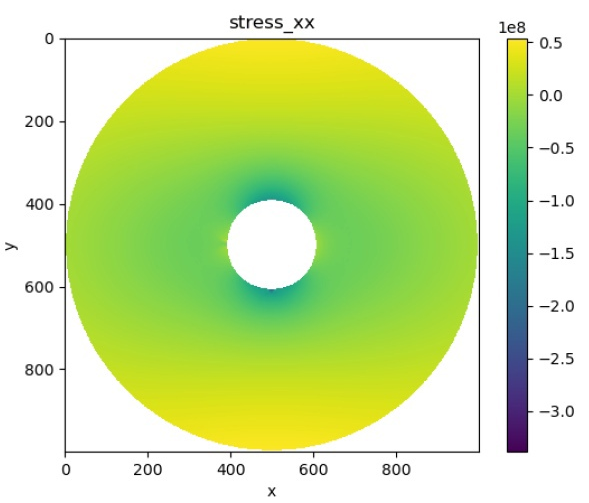
\includegraphics[width=\textwidth]{stressx_06tf}
	 		\subcaption{$t = 0.06t_f$}
	 	\end{subfigure}
	 	\qquad\qquad
	 	\begin{subfigure}[H]{0.38\textwidth}
	 		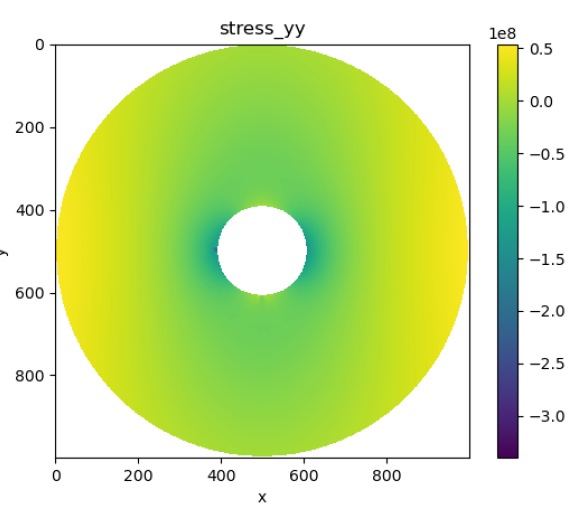
\includegraphics[width=\textwidth]{stressy_06tf}
	 			 		\subcaption{$t = 0.06t_f$}
	 	\end{subfigure}	
	 	\caption{Напряжения}
	 \end{figure}	
 
 При $t=0.2t_f$ происходит развитие 4-х трещин в топливной таблетке. Напряжение и деформации достигли пределов прочности $\sigma_f$ и $\varepsilon_f$. Функция памяти отклоняется от единицы, т.е. появляются анизотропные эффекты. 
  \begin{figure}[H]
 	\centering
 	\begin{subfigure}[H]{0.38\textwidth}
 		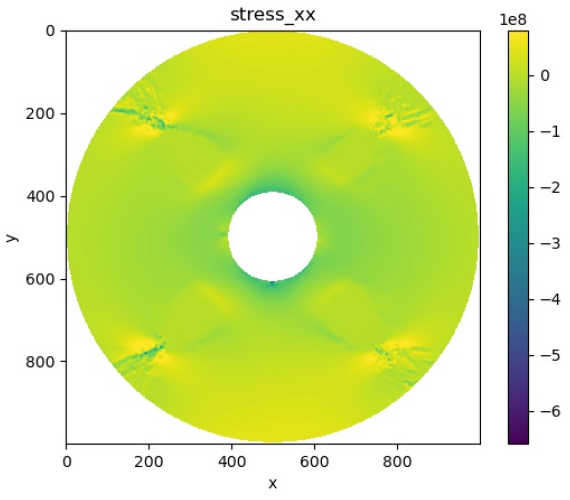
\includegraphics[width=\textwidth]{stressx_002}
 			 		\subcaption{$t = 0.2t_f$}
 	\end{subfigure}
 	\qquad\qquad
 	\begin{subfigure}[H]{0.38\textwidth}
 		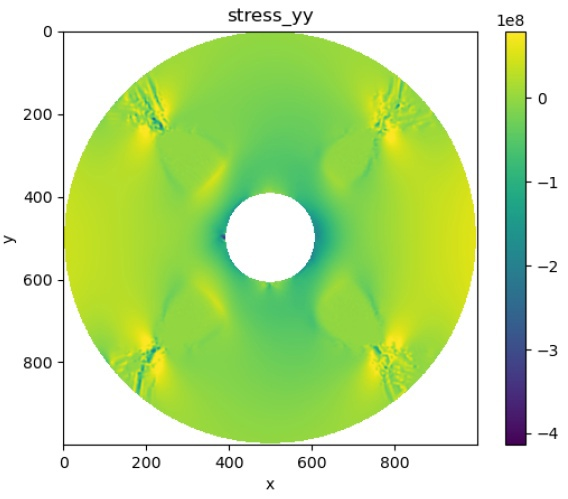
\includegraphics[width=\textwidth]{stressy_002}
 			 		\subcaption{$t = 0.2t_f$}
 	\end{subfigure}	
 	\caption{Напряжения}
 \end{figure}	

При $t=0.9t_f$ разрушение продолжается, появляются новые трещины. Многие деформации достигли	значение $\varepsilon_0$, при котором материал не способен передавать напряжения в направлении, ортогональном трещине.
 \begin{figure}[H]
	\centering
	\begin{subfigure}[H]{0.38\textwidth}
		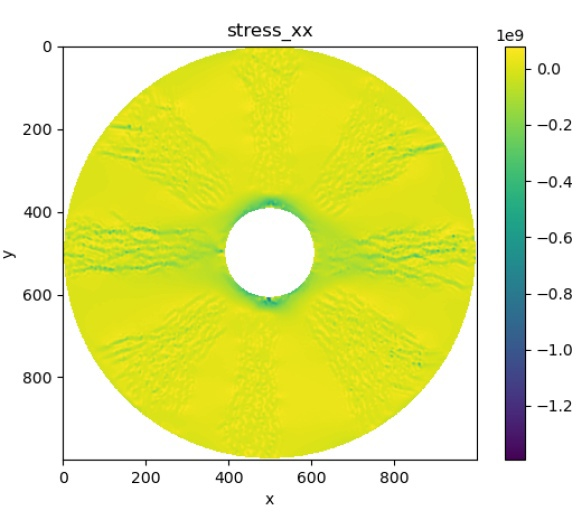
\includegraphics[width=\textwidth]{stressx_2tf}
			 		\subcaption{$t = 0.9t_f$}
	\end{subfigure}
	\qquad\qquad
	\begin{subfigure}[H]{0.38\textwidth}
		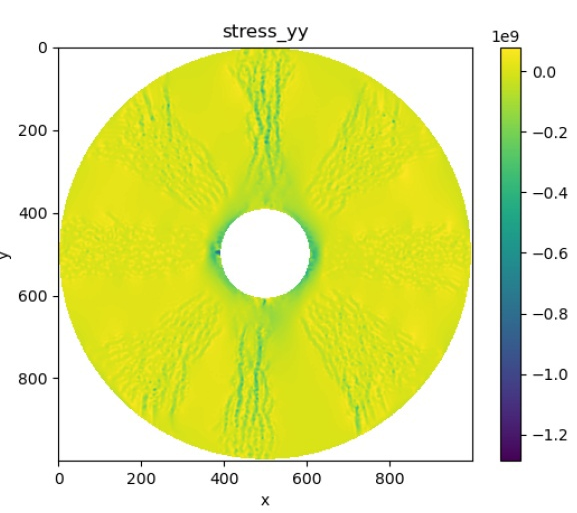
\includegraphics[width=\textwidth]{stressy_2tf}
			 		\subcaption{$t = 0.9t_f$}
	\end{subfigure}	
	\caption{Напряжения}
\end{figure}	

При $t=t_f$ видно большое количество трещин по 8 направлениям. При появлении трещин напряжения спадают практически до нуля, и на всех графиках не превышают предел прочности $\sigma_f$.
 \begin{figure}[H]
	\centering
	\begin{subfigure}[H]{0.38\textwidth}
		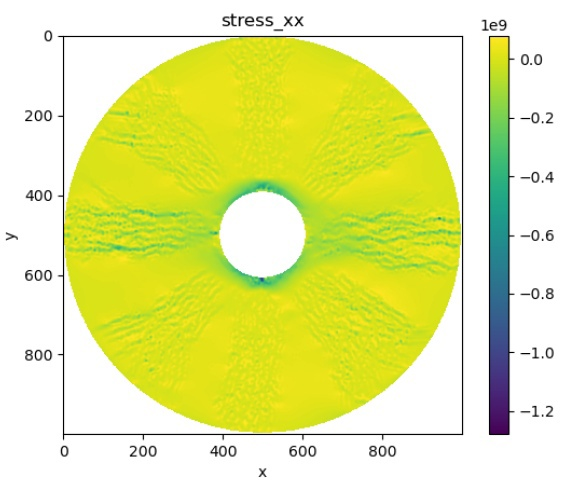
\includegraphics[width=\textwidth]{stressx_tf}
		\subcaption{$t = t_f$}
	\end{subfigure}
	\qquad\qquad
	\begin{subfigure}[H]{0.38\textwidth}
		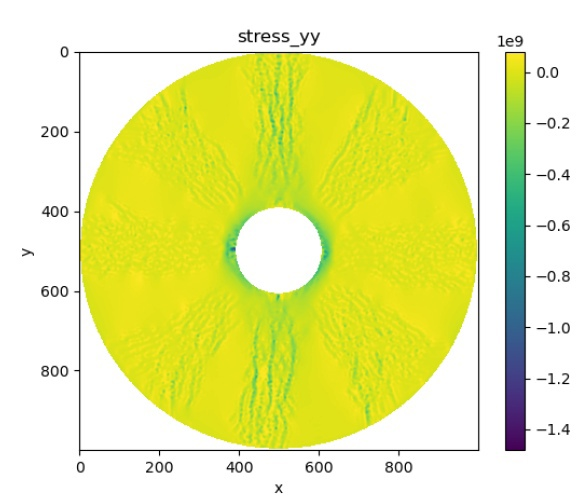
\includegraphics[width=\textwidth]{stressy_tf}
		\subcaption{$t = t_f$}
	\end{subfigure}	
	\caption{Напряжения}
\end{figure}	
	
	\section-{Заключение}
%	В настоящей работе рассмотрена задача термоупругости для двумерного случая.
	Была исследована математическая модель разрушения пластины, состоящей из диоксида урана UO$_2$. Данная задача была решена методом конечных элементов на треугольной сетке. Для тестовой задачи подтвержден порядок точности схемы.
	
	Проведено математическое моделирование разрушения топливной таблетки в двумерной задаче, описывающей горизонтальное сечение. Применение описанной модели размазанных трещин приводит к непротиворечивым результатам.
	
	Решение вышеуказанной задачи было реализовано с помощью  библиотеки FEniCS на языке программирования <<Python>>.
	
	\pagebreak
	\begin{thebibliography}{1}
		\bibitem{kovalenko} \textit{Коваленко А.Д.} Основы термоупругости : учебное пособие / А.Д. Коваленко. -- Киев: Наукова думка, 1970. -- 307 с.
		\bibitem{frost} \textit{Фрост Б.} ТВЭЛы ядерных реакторов: пер. с англ. М.: Энергоатомиздат, 1986. --
		\mbox{248 с.}
		\bibitem{zienkevich} \textit{Зенкевич О., Морган К.} Конечные элементы и аппроксимация: Пер. с англ. -- М.: Мир, 1986. --  318 с.
		\bibitem{zarubin} \textit{Зарубин В.С., Кувыркин Г.Н.} Математические модели механики и электродинамики сплошной среды. -- М.: Изд-во МГТУ им. Н.Э. Баумана, 2008. -- 512 с.: ил. (Математическое моделирование в технике и в технологии).
		\bibitem{galanin1} \textit{Галанин М.П., Савенков Е.Б.} Методы численного анализа математических\\ моделей. М.: Изд-во МГТУ им. Н.Э. Баумана,	2010. 592 с.
		\bibitem{galanin2} Математическое моделирование разрушения хрупкого материала под действием тепловых нагрузок / М.П. Галанин [и др.] // Препринты ИПМ им. М.В. Келдыша. 2013. № 100. 36 с. URL:
		http://library.keldysh.ru/preprint.asp?id=2013-100.
		\bibitem{smeared crack} \textit{ Dahlblom O., Ottosen N.S.} Smeared Crack Analysis of Concrete Using a	Nonlinear Fracture Model // Fracture Mechanics of Concrete. Nordiс Seminar Held at Division of Building Materials, November 6, 1986, p. 31-46.
		
		
	\end{thebibliography}
	
	
\end{document}
